\section{}
% Wyznaczyć średni czas propagacji impulsu przez bramkę mierząc okres drgań generatora zbudowanego z trzech bramek. Użyć do budowy generatora bramek serii podstawowej 7400. a potem bramek serii szybkiej 74S00. Porównaj wyniki.

Wyznaczono średni czas propagacji impulsu przez bramkę mierząc okres drgań generatora zbudowanego z trzech bramek NAND.
Do budowy generatora najpierw wykorzystano układ 7400, a następnie układ 74S00.
Uzyskane pomiary pomnożono przez \(\frac{1}{2*3}\), co dało czasy propagacji dla 7400 i 74S00 wynoszące odpowiednio \(10.38\)ns oraz \(3.5\)ns.
Czasy te zawierają się w zakresie dopuszczalnych wartości określonych w notach katalogowych układów.

\begin{figure}[H]
    \centering
    \begin{circuitikz}
        \draw
        (0, 0) node(gate1)[nand port] {}
        (2, 0) node(gate2)[nand port] {}
        (4, 0) node(gate3)[nand port] {};

        \draw
        (gate2.in 1) to[short,-] (gate2.in 2)
        (gate2.in 1 |- gate2.out) to[short,*-] (gate1.out);

        \draw
        (gate3.in 1) to[short,-] (gate3.in 2)
        (gate3.in 1 |- gate3.out) to[short,*-] (gate2.out);

        \draw
        (gate3.out) to[short,-*] ++(1, 0) coordinate (cen);

        \draw
        (gate1.in 1) to[short,-] (gate1.in 2)
        (gate1.in 1 |- gate1.out) to[short,*-] ++(-1, 0)
        to[short,-] ++(0, 1)
        to[short,-] (cen |-, 1)
        to[short,-] (cen);

        \draw
        (cen) to[short,-*] ++(1, 0)
        node[anchor=west] {$U_{wy}$};
    \end{circuitikz}
    \caption{Schemat układu generatora.}
\end{figure}

\begin{figure}[H]
    \centering
    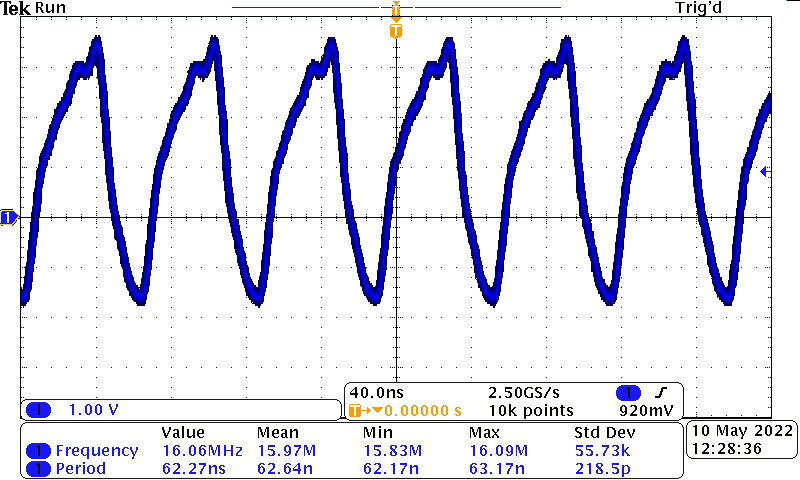
\includegraphics[width=\textwidth]{include/4/1.png}
    \caption{Pomiar okresu drgań generatora zbudowanego przy pomocy układu 7400.}
\end{figure}

\begin{figure}[H]
    \centering
    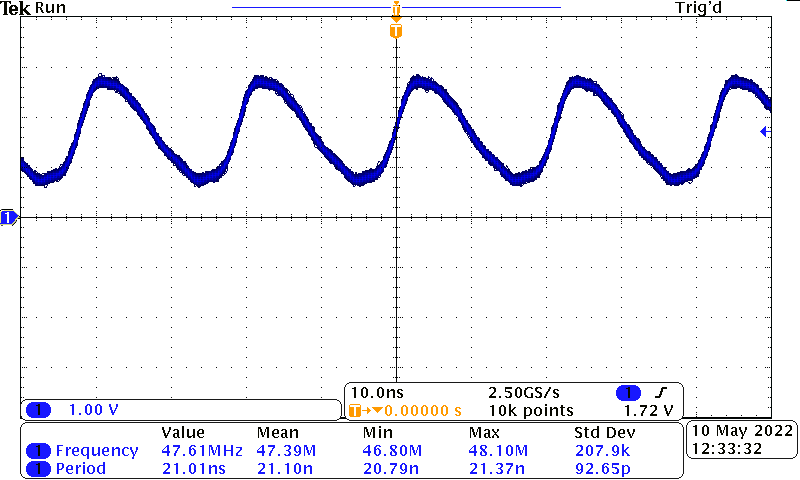
\includegraphics[width=\textwidth]{include/4/2.png}
    \caption{Pomiar okresu drgań generatora zbudowanego przy pomocy układu 74S00.}
\end{figure}